\documentclass{amsart}

%%%%%%%%%%%%%%%%%%%%%%%%%%%%%%%%%%%%%%

\usepackage[utf8]{inputenc}
\usepackage[T1]{fontenc}

\usepackage{a4wide}%en grand
\usepackage{changepage}%indentation

\usepackage{xcolor}
\usepackage{amsfonts,amsthm,amssymb,amsmath}
\usepackage{mathtools}
\usepackage{wasysym}
\usepackage{xspace}
\usepackage{graphicx}
%\usepackage[notcite,notref]{showkeys} % shows labels 
\usepackage{breqn}
\usepackage{algorithm}
\usepackage{algorithmic}
\usepackage{tabularx}

\usepackage[english]{babel} %gestion des langues
\usepackage{caption}
\usepackage{subcaption}
\usepackage{paralist}
\usepackage{multirow}

\usepackage{hyperref}
\hypersetup{colorlinks=true, citecolor=darkblue, linkcolor=darkblue}
\usepackage{hypcap}

\usepackage[noabbrev,capitalise]{cleveref}
\usepackage{autonum}
\usepackage{xspace}

%%%%%%%%%%%%%%%%%%%%%%%%%%%%%%%%%%%%%%

\newtheorem{theorem}{Theorem}[section]
\newtheorem{proposition}[theorem]{Proposition}
\newtheorem{lemma}[theorem]{Lemma}
\newtheorem{ce}[theorem]{Counter-example}
\newtheorem{claim}[theorem]{Claim}
\newtheorem{corollary}[theorem]{Corollary}
\newtheorem{definition}[theorem]{Definition}
\newtheorem{notation}[theorem]{Notation}
\theoremstyle{remark}
\newtheorem{remark}{Remark}[section]
\newtheorem{example}{Example}
\newtheorem{algo}{Algorithm}
\newtheorem*{example*}{Example}

\crefname{theorem}{Theorem}{Theorems}
\crefname{lemma}{Lemma}{Lemmas}

\definecolor{darkblue}{rgb}{0,0,0.7} % darkblue color
\newcommand{\darkblue}{\color{darkblue}} % darkblue command
\newcommand{\defn}[1]{\textsl{\darkblue #1}} % emphasis of a definition

%%%%%%%%%%%%%%%%%%%%%%%%%%%%%%%%%%%%%%

\newcommand*{\dual}[1]{{#1^*}}
\newcommand*{\nbd}[0]{neighbourhood\xspace}
\newcommand*{\ef}[0]{E-finite\xspace}
\newcommand*{\vf}[0]{V-finite\xspace}
\newcommand*{\ktg}[0]{$k$-triangulation\xspace}

\newcommand{\cl}{\prec}
\newcommand{\cle}{\preccurlyeq}

\newcommand{\surface}{\mathcal{S}}

\newcommand{\set}[2]{\left\{ #1 \;\middle|\; #2 \right\}} % set notation
\newcommand{\bigset}[2]{\big\{ #1 \;\big|\; #2 \big\}} % big set notation
\newcommand{\Bigset}[2]{\Big\{ #1 \;\Big|\; #2 \Big\}} % Big set notation
\newcommand{\setangle}[2]{\left\langle #1 \;\middle|\; #2 \right\rangle} % set notation
\newcommand{\ssm}{\smallsetminus} % small set minus
\newcommand{\dotprod}[2]{\left\langle \, #1 \; \middle| \; #2 \, \right\rangle} % dot product
\newcommand{\symdif}{\,\triangle\,} % symmetric difference
\newcommand{\one}{{1\!\!1}} % the all one vector
\newcommand{\eqdef}{\mbox{\,\raisebox{0.2ex}{\scriptsize\ensuremath{\mathrm:}}\ensuremath{=}\,}} % :=
\newcommand{\defeq}{\mbox{~\ensuremath{=}\raisebox{0.2ex}{\scriptsize\ensuremath{\mathrm:}} }} % =:
\newcommand{\viceversa}{\textit{vice versa}} % vice versa

\graphicspath{{../figures/}}

% marginal comments
\usepackage{todonotes}
\newcommand{\vincent}[1]{\todo[color=blue!30]{#1 \\ \hfill --- V.}}
\newcommand{\mathias}[1]{\todo[color=red!30]{#1 \\ \hfill --- M.}}

%%%%%%%%%%%%%%%%%%%%%%%%%%%%%%%%%%%%%%

\title[Infinite multitriangulations and multitriangulations of surfaces]{Infinite multitriangulations \\ and multitriangulations of surfaces}

\thanks{ML was partially supported by the French ANR grant GATO~(16\,CE40\,0009). \\ \indent VP was partially supported by the French ANR grants SC3A~(15\,CE40\,0004\,01) and CAPPS~(17\,CE40\,0018).}

\author{Mathias Lepoutre}
\address{LIX, \'Ecole Polytechnique, Palaiseau}
\email{mathias.lepoutre@lix.polytechnique.fr}
\urladdr{\url{http://www.lix.polytechnique.fr/Labo/Mathias.Lepoutre/}}

\author{Vincent Pilaud}
\address{CNRS \& LIX, \'Ecole Polytechnique, Palaiseau}
\email{vincent.pilaud@lix.polytechnique.fr}
\urladdr{\url{http://www.lix.polytechnique.fr/~pilaud/}}

%%%%%%%%%%%%%%%%%%%%%%%%%%%%%%%%%%%%%%

\begin{document}

\begin{abstract}
We extend previous work on the structure of $k$-stars of a multi-triangulation on a convex polygon to the case of multi-triangulations on any surface, orientable or not. 

To that extent, we use the universal cover construction, that makes a map on a surface into a periodic map of an infinite polygon. We generalize the work of Pilaud and Santos to multi-triangulation of an infinite polygon, with some additional constraints, and then conclude about the case of multi-triangulations on any surface.
\end{abstract}

\maketitle

\begin{figure}[h]
	\capstart
	\centerline{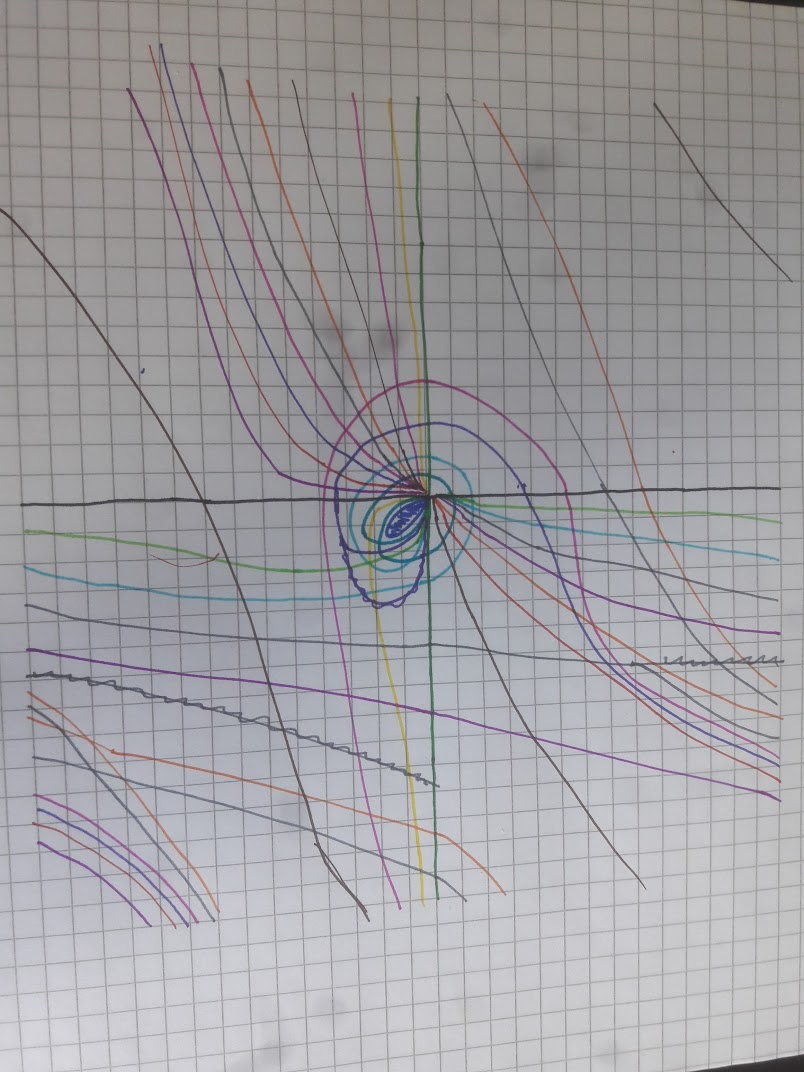
\includegraphics[scale=.42]{torus}}
	\caption{A $2$-triangulation of a torus with a hole.}
	\label{fig:torus}
\end{figure}


\section{Multitriangulations of infinite polygons}

\subsection{Infinite polygons}

\begin{definition}
A \defn{polygon}~$P$ is a cyclically ordered set, that might be finite or infinite.
We write~$a \cl b \cl c$ for the cyclic order.
The elements of~$P$ are called \defn{points} and pairs of elements of~$P$ are called \defn{diagonals}.
For two points~$a,b \in P$, let~$[a,b] \eqdef \set{c \in P}{a \le c \le b}$, and define similarly the intervals~$[a,b[$, $]a,b]$ and~$]a,b[$ (with open brackets for strict inequalitites).
Two diagonals~$(a,c)$ and~$(b,d)$ of~$P$ \defn{cross} if~$a \cl b \cl c \cl d$.
\end{definition}

\begin{definition}
If $x$ and $y$ are two points of a polygon~$P$ such that the interval~$]x,y[$ is empty, we say that~$x$ is the \defn{predecessor} of~$y$ and that~$y$ is the \defn{successor} of~$x$. A polygon~$P$ is \defn{tidy} if each point of~$P$ has both a predecessor and a successor. In particular, finite polygons are tidy.
\end{definition}

\begin{definition}
A set~$X$ of diagonals of a polygon~$P$ is 
\begin{itemize}
\item \defn{\ef} if each diagonal of~$X$ is crossed by a finite number of diagonals of~$X$,
\item \defn{\vf} if each vertex of~$P$ is incident to finitely many diagonals of~$X$.
\end{itemize}
\end{definition}

\begin{definition}[periodic]

\end{definition}

\subsection{Infinite multitriangulations}

\begin{definition}
A \defn{$k$-crossing} of a polygon~$P$ is a set of~$k$ pairwise crossing diagonals of~$P$.
A \defn{$k$-triangulation} of~$P$ is an inclusion maximal set of diagonals of~$P$ with no $(k+1)$-crossing.
\end{definition}

\begin{definition}
The \defn{length} of a diagonal~$(a,b)$ of a polygon~$P$ is the minimum~$\ell(a,b)$ of~$|{]a,b[}|$ and~$|{]b,a[}|$ (note that this might be infinite).
A diagonal~$(a,b)$ with~$\ell(a,b) > k$ (resp.~$\ell(a,b) = k$, resp.~$\ell(a,b) < k$) is a \defn{$k$-relevant} (resp.~\defn{$k$-boundary}, resp.~\defn{$k$-irrelevant}) diagonal.
\end{definition}

\begin{remark}
Observe that a diagonal contained in a $(k+1)$-crossing must be $k$-relevant.
Therefore, any \ktg contains all $k$-irrelevant and $k$-boundary diagonals by maximality.
\end{remark}


\begin{definition}
A \defn{$k$-star} of a polygon~$P$ is a set of diagonals of~$P$ of the form~$\set{(s_i, s_{i+k})}{0 \le i \le 2k}$ where~$s_0 \cl \dots \cl s_{2k}$ (the indices are understood modulo~$2k+1$).
\end{definition}

\begin{definition}
An \defn{angle} of a set~$X$ of diagonals of a polygon~$P$ is a pair of diagonals~$\{(u,v), (v,w)\}$ with~$u \cl v \cl w$ such that~$X$ contains no diagonal of the form~$(v,t)$ with~$w \cl t \cl u$. The angle is denoted by~$\angle(u,v,w)$ and we say that~$v$ is the \defn{apex} of~$\angle(u,v,w)$. An angle is \defn{$k$-relevant} if none of its diagonals is $k$-irrelevant. A set~$Y$ of diagonals of~$P$ crosses the angle~$\angle(u,v,w)$ if each diagonal of~$Y$ crosses both~$(u,v)$ and~$(v,w)$.
\end{definition}

One of the objectives of this paper is to prove the following structural results on infinite multitriangulations

\begin{theorem}
\label{thm:structureInfinite}
Let~$T$ be a \ef \ktg of a tidy polygon~$P$.
\begin{enumerate}
\item Each $k$-relevant angle of~$T$ is contained in precisely one $k$-star of~$T$.
\item Each $k$-relevant (resp.~$k$-boundary, resp.~$k$-irrelevant) diagonal of~$P$ is contained in precisely two (resp.~one, resp.~none) $k$-stars of~$T$.
\item For any $k$-relevant diagonal~$e$ of~$T$, there exists a unique diagonal~$f$ not in~$T$ such that~$T \symdif \{e,f\}$ is another $k$-triangulation. The diagonal~$f$ only depend on the two $k$-stars of~$T$ containing~$e$.
\item Let~$P'$ denote a polygon obtained by replacing $k+1$ consecutive points of~$P$ by~$k$ points. Then there exists a flattening (resp.~inflating) operation that transforms the \ktg{}s of~$P$ into the \ktg{}s of~$P'$ (resp.~and \viceversa).
\item For any point~$p$ of the plane, the $k$-depth of~$p$ in~$P$ is equal to the sum of the winding numbers around~$p$ of the $k$-stars of~$T$.
\vincent{Vrai ?}
\end{enumerate}
\end{theorem}

\begin{remark}
\begin{itemize}
\item flip graph connected? Increasing flip graph?
\item duality with pseudoline arrangements?
\item $k$-arboresence? connection to $k$-edge-connected but not locally $(k+1)$-edge-connected.
\end{itemize}
\end{remark}

\section{Multitriangulations of surfaces}

\begin{definition}
Consider an connected surface~$\surface$ with boundary and a set~$V$ of marked points on the boundary, with at least one marked point on each boundary component. An \defn{arc} of~$\surface$ is a curve on~$\surface$ connecting two points of~$V$ and whose interior is disjoint from the boundary of~$\surface$. We consider arcs up to homotopy relative to their endpoints in~$\surface$ and we disallow arcs homotopic to a boundary segment of~$\surface$.
\end{definition}

\begin{definition}
Universal cover~$\pi : \bar\surface \to \surface$.
\vincent{Not clear}
\end{definition}

\begin{definition}
A \defn{$k$-crossing} on~$\surface$ is a collection~$\alpha_1, \dots, \alpha_k$ of $k$ arcs of~$\surface$ which admit pairwise crossing representatives~$\bar\alpha_1, \dots, \bar\alpha_k$ in the universal cover~$\bar\surface$.
A \defn{$k$-triangulation} of~$P$ is an inclusion maximal set of diagonals of~$P$ with no $(k+1)$-crossing.
\end{definition}

\begin{remark}
Be careful: a $k$-crossing on~$\surface$ is NOT a collection of pairwise crossing arcs of~$\surface$. Namely, there are collections of pairwise crossing arcs of~$\surface$ which do not admit pairwise crossing representatives. The simplest examples are self-crossing arcs, since their representative are not self-crossing. Further examples are given in \cref{fig:notkcrossing}.
\vincent{Todo.}
\end{remark}

\begin{theorem}
\label{thm:structureSurface}
Any \ktg of a surface of genus~$g$ with~$b$ boundaries and~$n$ marked points has precisely $n + 2k(2g + b - 2)$ $k$-stars and $kn + k(2k + 1)(2g + b - 2)$ $k$-relevant arcs.
\end{theorem}


\begin{remark}
\begin{itemize}
\item \cite[Lem.~7.10]{PilaudSantos}: Any $k$-triangulation of the $n$-gon contains at most $k(n-2p-1)$ $p$-relevant diagonals. Extension for surfaces.
\item flip graph connected? Increasing flip graph?
\item duality? Line space of the surface?
\item punctures?
\end{itemize}
\end{remark}

\section{Proof of \cref{thm:structureInfinite}}

\subsection{$(k-1)$-crossings crossing an angle}

\begin{lemma}
In a \ktg of a tidy polygon, any $k$-relevant angle is crossed by a $(k-1)$-crossing.
\end{lemma}
\begin{proof}
Any angle~$\angle(u,v,w)$ is crossed by the $(k-1)$-crossing~$\set{(v-k+i, v+i)}{i \in [k-1]}$ of $k$-boundary diagonals, which belongs to the \ktg.
\end{proof}

\begin{definition}
Let $\angle(u,v,w)$ be a $k$-relevant angle of $T$ and let $(a, a')$ and $(b ,b')$ be two diagonals of $T$ that cross $\angle(u,v,w)$ such that $u \cl a \cl v \cl a' \cl w$ and $u \cl b \cl v \cl b' \cl w$. we say that $(a, a')$ is \defn{$v$-farther} than $(b, b')$ if $u \cl a \cle b \cl v \cl b' \cle a' \cl w$. Let $A = \{(a_1, a'_1), \dots, (a_{k-1}, a'_{k-1})\}$ and $B = \{(b_1, b'_1), \dots,(b_{k-1}, b'_{k-1})\}$ be two $(k-1)$-crossings that cross $\angle(u,v,w)$ such that $u \cl a_1 \cl a_2 \cl \dots \cl a_{k-1} \cl v \cl a'_1 \cl a'_2 \cl \dots \cl a'_{k-1} \cl w$ and $u \cl b_1 \cl b_2 \cl \dots \cl b_{k-1} \cl v \cl b'_1 \cl b'_2 \cl \dots \cl b'_{k-1} \cl w$. Then we say that $A$ is \defn{$v$-farther} than $B$ if $(a_i, a'_i)$ is $v$-farther than $(b_i, b'_i)$ for every $i \in [k-1]$. We say that $A$ is the \defn{$v$-farthest} $(k-1)$-crossing if it is $v$-farther than any other $(k-1)$-crossing crossing~$\angle(u,v,w)$.
\end{definition}

\begin{lemma}
In a \ktg, the set of $(k-1)$-crossings crossing a given $k$-relevant angle forms a distributive lattice.
\end{lemma}
\begin{proof}
Let $A = \{(a_1, a'_1), \dots, (a_{k-1}, a'_{k-1})\}$ and $B = \{(b_1, b'_1), \dots,(b_{k-1}, b'_{k-1})\}$ be two $(k-1)$-crossings crossing the angle $(u,v,w)$.

There is no $i$ such that $(a_i, a'_i)$ crosses $(b_i, b'_i)$. 
Indeed, suppose $a_i \cl b_i \cl v \cl a'_i \cl b'_i$. Then $\{(u, v), (a_1, a'_1), \dots, (a_i, a'_i), (b_i, b'_i), \dots, (b_{k-1}, b'_{k-1})\}$ forms a $(k+1)$-crossing. 
Similarly, if $b_i \cl a_i \cl v \cl b'_i \cl a'_i$, then $\{(u, v), (b_1, b'_1), \dots, (b_i, b'_i), (a_i, a'_i), \dots, (a_{k-1}, a'_{k-1})\}$ forms a $(k+1)$-crossings.
Hence $A$ and $B$ are edgewise comparable.

We define the meet (resp.~join) of $A$ and $B$ as their edgewise minimum (resp.~maximum). With this definition it is easy to see that we obtain a distributive lattice.
\end{proof}

\begin{lemma}
In a \ktg, for any angle~$\angle(u,v,w)$ crossed by at least one $(k-1)$-crossing, there exists a $v$-farthest $(k-1)$-crossing crossing~$\angle(u,v,w)$.
\end{lemma}
\begin{proof}
By \ef{}ness, the angle~$\angle(u,v,w)$ is crossed by a finite number of $(k-1)$-crossings. Hence the distributive lattice of such $(k-1)$-crossings is finite, and has a unique maximum.
\end{proof}

\begin{corollary}
In a \ktg of a tidy polygon, for any angle~$\angle(u,v,w)$, there exists a $v$-farthest $(k-1)$-crossing crossing~$\angle(u,v,w)$.
\end{corollary}


\subsection{any angle belongs to a $k$-star}

\begin{lemma}
In a \ktg, any angle which is maximally crossed by a $(k-1)$-crossing belongs to a $k$-star.
\end{lemma}
\begin{proof}
cf thm4.1 of  Pilaud Santos, but to be rewritten.





Let $E=\{(e_1,e'_1), \cdots , (e_{k-1},e'_{k-1})\}$ be a $(k - 1)$-crossing intersecting $\angle(u, v, w)$ and assume that it is $v$-maximal. 
We will prove that the diagonals $(u, e'_1),(e_1, e'_2)\cdots(e_{k-2}, e'_{k-1}), (e_{k-1}, w)$ are in $T$ such that the points $u$, $e_1,\cdots,e_{k-1}$, $v$, $e'_1,\cdots,e'_{k-1}$, $w$ are the vertices of a $k$-star of $T$ containing the angle $\angle(u, v, w)$. 

<<<<<<< HEAD
To get this result, we use two steps: first we prove that $\angle(e_1, e'_1, u)$ is an angle of $T$, and then we prove that the edges $(e_2,e'_2),\cdots, (e_{k-1},e'_{k-1}), (v, w)$ form a $(k-1)$-crossing intersecting $\angle(e_1, e'_1, u)$ and $e'_1$-maximal (so that we can reiterate the argument).

{\bf First step.}
Suppose that $(u, e'_1)$ is not in $T$. 
Since $T$ is a triangulation, there is a $k$-crossing $F=\{(f_1, f'_1),\cdots, (f_k, f'_k)\}$ (with $u \cl f_1 \cl \cdots \cl f_k \cl e'_1 \cl f'_1 \cl \cdots \cl f'_k \cl u$) that prevents the edge $(u, e'_1)$.
=======
To get this result, we use two steps: first we prove that $\angle(e_1, e'_1, u)$ is an angle of $T$, and then we prove that the diagonals $e_2,\cdots, e_{k-1}, (v, w)$ form a $(k-1)$-crossing intersecting $\angle(e_1, e'_1, u)$ and $e'_1$-maximal (so that we can reiterate the argument).

{\bf First step.}
Suppose that $(u, e'_1)$ is not in $T$. 
Since $T$ is a triangulation, there is a $k$-crossing $F=(f_1, f'_1),\cdots, (f_k, f'_k)$ that prevents the diagonal $(u, b1)$, so that: $u \cl f_1 \cl \cdots \cl f_k \cl e'_1 \cl f'_1 \cl \cdots \cl f'_k \cl u$.
>>>>>>> dead106192b2d8786fef886effffa436c0b2fcb6

Note first that $f_k \in [v,e'_1[$. Indeed, if $f_k \in ]u, v[$, then $F \cup \{(u, v)\}$ forms a $(k + 1)$-crossing.
Note also that $f'_k \in ]f'_{k-1},w]$. Indeed, if it is not the case, then $f'_k \in ]w, u[$, and $f_k \neq v$, because $\angle(u, v, w)$ is an angle, and $E \cup \{(v,w),(f_k, f'_k)\}$ forms a $(k + 1)$-crossing. 
Consequently, we have $e'_1 \cl f'_1 \cl \cdots \cl f'_{k-1} \cl w$.

Let $\ell = \text{max}\set{j\in[k-1]}{\forall i\in[j],e'_i \cl f'_i \cl w}$.
Then for any $i\in[\ell]$, since $\{(e_1,e'_1), \cdots , (e_i,e'_i)\} \cup \{(f_i,f'_i), \cdots , (f_k,f'_k)\}$ does not form a $(k + 1)$-crossing, we have $f_i \in ]u, e_i]$. 
Thus for any $i\in[\ell]$, $u \cl f_i \cle e_i \cl v \cl e'_i \cl f'_i \cl w$, so that $f_i$ is $v$-farther than $e_i$.
Furthermore, we have $u \cl f_1 \cl \cdots \cl f_\ell \cl e_{\ell+1} \cl \cdots \cl e_{k-1} \cl v \cl f'_1 \cl \cdots \cl f'_\ell \cl e'_{\ell+1} \cl \cdots \cl e'_{k-1} \cl w$. 
Consequently, we get a $(k - 1)$-crossing $\{f_1, \cdots , f_\ell
, e_{\ell+1}, \cdots , e_{k-1}\}$ which is $v$-farther than $\{e_1, \cdots , e_{k-1}\}$; this contradicts the definition of $\{e_1, \cdots , e_{k-1}\}$. 
Thus we obtain: $(u, e'_1) \in  T$.

Suppose now that $\angle(e_1, e'_1, u)$ is not an angle of $T$. 
Then there exists $e_0 \in ]u, e_1[$ such that $(e'_1, e_0) \in  T$. 
But then the $(k - 1)$-crossing $\{(e_0, e'_1), (e_2,e'_2), \cdots , (e_{k-1},e'_{k-1})\}$ is $v$-farther than $E$. 
This implies that $\angle(e_1, e'_1, u)$ is an angle of $T$.



{\bf Second step.}
<<<<<<< HEAD
Let $F=\{(f_2,f'_2), \cdots , (f_{k},f'_{k})\}$ (with $e_1 \cl f_2 \cl \cdots \cl f_{k} \cl e'_1 \cl f'_2 \cl \cdots \cl f'_{k} \cl u$) be a $(k - 1)$-crossing intersecting $\angle(e_1, e'_1, u)$ and $e'_1$-farther than the $(k-1)$-crossing $\{(e_2,e'_2), \cdots , (e_{k-1},e'_{k-1}), (v, w)\}$.
=======
Let $F$ be a $(k - 1)$-crossing intersecting $\angle(e_1, e'_1, u)$ and $e'_1$-farther than the $(k-1)$-crossing $\{e_2, \cdots , e_{k-1}, [v, w]\}$. 
Let $f_2 = [f_2, f'_2], \cdots , f_k = [f_k, f'_k]$ denote its diagonals, with $e_1 \cl f_2 \cl \cdots \cl f_k \cl e'_1 \cl f'_2 \cl \cdots \cl f'_k \cl u$.
>>>>>>> dead106192b2d8786fef886effffa436c0b2fcb6

Note first that $f'_{k} = w$. 
Indeed, if it is not the case, then $f'_{k} \in ]w, u[$ (because $(f_k,f'_k)$ is $e'_1$-farther than $(v,w)$), and $f_{k} \in ]u,v[$ (because $\angle(u, v, w)$ is an angle, and $(f_k,f'_k)$ is $e'_1$-farther than $(v,w)$).
Thus either $f_k \in ]e_1, v[$ and then $F \cup \{(u, v), (e_1,e'_1)\}$ forms a $(k + 1)$-crossing, or $f_k \in ]v, e'_1[$ and then $E \cup \{(v,w),(f_k, f'_k)\}$ forms a $(k + 1)$-crossing. 
Consequently, we have $e'_1 \cl f'_2 \cl \cdots \cl f'_{k-1} \cl w$.

Furthermore, for any $i\in[2,k-1]$, $(f_i,f'_i)$ is $e'_1$-farther than $(e_i,e'_i)$, so that $e_1 \cl f_i \cle e_i \cl e'_1 \cl e'_i \cle f'_i \cl u$. 
In particular, $e_1 \cl f_{k-1} \cle e_{k-1} \cl v$ and we get $u \cl e_1 \cl f_2 \cl \cdots \cl f_{k-1} \cl v \cl e'_1 \cl f'_2 \cl \cdots \cl f'_{k-1} \cl w$.
Consequently, the $(k - 1)$-crossing $\{(e_1,e'_1), (f_2,f'_2), \cdots , (f_{k-1},f'_{k-1})\}$ is $v$-farther than $E$, which is a contradiction.











\end{proof}

We may need the \ktg to be \vf?

\subsection{any diagonal belongs to $2$ $k$-stars, and can be flipped}

\begin{lemma}
When $k\geq 2$, any \ef \ktg of a \nbd is \vf.
\end{lemma}
\begin{proof}
Any diagonal of the $k$-border surrounding a given vertex intersects all diagonals adjacent to this vertex.
\end{proof}

\begin{lemma}
Any diagonal of a \vf \ktg belongs to $4$ angles.
\end{lemma}
\begin{proof}
The vertices adjacent to the diagonal have finite degree. Take the neighbours just before and after the other vertex. The $4$ hereby obtained diagonals form angles with the first one.
\end{proof}

\begin{lemma}
Any diagonal adjacent to $2$ $k$-star can be flipped.
\end{lemma}
\begin{proof}
cf Pilaud Santos. to be adapted to the infinite case, but shouldn't need any additional hypothesis. quite long though : section 3.
\end{proof}

\section{More}

\subsection{more lemmas}

\begin{lemma} 
Any diagonal of a \ef \ktg of a \nbd belongs to 4 angles. 
\end{lemma}
\begin{proof}
see direct proof on sheet.
\end{proof}

\subsection{some counter-examples}

\begin{ce}
The polygon of a periodic \ktg is not necessarily a \nbd.
\end{ce}
\begin{proof}

\end{proof}

\begin{ce}
A periodic \ef \ktg may have angles that are not crossed by a $(k-1)$-crossing.
\end{ce}
\begin{proof}

\end{proof}

\begin{ce} 
A periodic \ktg may not be \ef.
\end{ce}
\begin{proof}

\end{proof}

\begin{ce}
A \ef \ktg of a \nbd is not necessarily \vf.
\end{ce}
\begin{proof}
k=1
\end{proof}



\bibliographystyle{abbrv}
\bibliography{../bibliography}

\end{document}
